\chapter{Evaluation}

In order to answer the questions raised in the introduction, the library \code{lox} is evaluated in this chapter.
This is done by, for example, comparing the execution speeds of \code{lox}, OpenMesh and PMP in several different benchmarks.
Furthermore, example code written with these three libraries is compared.  TODO: write this better.

Already during development, \code{lox}'s capabilities and ease of use were constantly tested by writing example programs and other tools.
As mentioned in the previous chapter, the command line utility \code{lox-cli} is developed alongside the main library to make sure the library offers all features such an application might require from it.
Additionally, an experimental application for rendering polygon meshes to SVG\footnote{Scalable Vector Graphic} files was developed outside of the main project, also assessing \code{lox}'s capabilities.
That application is not technically part of this master's thesis, but was used to create the images of meshes in this report, meaning they are all vector instead of pixel graphics.


\section{Execution Speed}

Geometry processing often has to deal with very large meshes, making the performance of geometry processing libraries very important.
Additionally, comparing the speed of \code{lox} to existing libraries is necessary in order to determine whether the abstractions employed by \code{lox} can be used without runtime overhead.
This chapter presents and discusses a number of different benchmarks.

All benchmarks were performed on a completely idle \textsf{Thinkpad T-460p} which, as already mentioned in chapter~4, contains an \textsf{Intel i7-6700\,HQ} and runs \textsf{Ubuntu 18.04}.
Of course, the notebook was \emph{not} running on battery during the benchmarks.
Additionally, at all times during the benchmarks, plenty of free main memory was available.
Each benchmark first executes the to be measured code 20~times as a warm-up without measuring anything.
Afterwards, the code is repeated 100 times and each iteration is measured individually.
From the 100 measured durations, the mean and standard deviation are calculated.

As already mentioned, the code, test meshes and raw results of all benchmarks can be found here: \url{https://github.com/LukasKalbertodt/masters-thesis}.

%TODO: Mention that DEM is not yet as optimized as it can be


\newpage
\subsection{Input/Output}

Some kind of IO can be found in most applications dealing with meshes, usually as the first and last step of said program.
While it is certainly not a particularly interesting processing step, its performance still is important to consider.
Different IO benchmarks were executed, covering this parameter space:

\begin{itemize}
  \item \textbf{Library/mesh implementation}: PMP, OpenMesh, \code{lox}'s half edge mesh (HEM), \code{lox}'s directed edge mesh (DEM) and \code{lox}'s shared vertex mesh (SVM) were tested.
  OpenMesh's and \code{lox}'s HEM were both configured for pure triangle meshes.
  \item \textbf{File format}: \textsc{Stl} and \textsc{Ply}.
  All benchmarks use little endian binary encoding.
  ASCII encoding only makes sense for tiny meshes in situations where it is necessary to manually inspect mesh data.
  Binary encoding is far more memory efficient and faster to read and write (independent of library).
  \item \textbf{Read or Write}
  \item \textbf{Mesh size}: the triangle meshes \enquote{cat} (59,292 faces) and \enquote{tiger} (232,956 faces) were tested.
  See \code{benchmarks/data/README.md} in the thesis' repository for more details.
\end{itemize}

Performing IO benchmarks comes with a few additional challenges.
Most importantly, it does not make sense to test the speed of the actual hardware disk as this is has little to do with the code performance.
To avoid this problem, a RAM disk\footnote{An allocated part of the main memory which is mounted into the file system.} can be used to store the input mesh files and as a target for all write operations.
However, this is not optimal as IO operations still have to communicate with the operating system, adding some overhead.

A better solution is to have an in-memory writer and reader in the benchmarking code to avoid interactions with the file system alltogether.
Benchmarks with both strategies were implemented for OpenMesh and \code{lox}, revealing that the RAM disk is roughly 1\% -- 6\% slower for read benchmarks and approximately 20\% -- 70\% slower for write benchmarks.
Unfortunately, PMP does not support reading from and writing to non-file streams.
To obtain a fair comparison between all three libraries, the in-memory disk solution was used for the main benchmark.

The results of the benchmark -- shown in figure~\ref{fig:io-benchmark} -- indicate a few different things:

\begin{itemize}
  \item \code{lox} outperforms the other libraries in all IO tasks, often significantly.
  \item In the \emph{read} benchmarks, \code{lox}'s HEM and DEM perform approximately equally well, with the SVM being notably faster.
  In the \emph{write} benchmarks however, the DEM performs as well as the SVM with the HEM being notably slower.
  This suggest that the DEM has the same speed as the HEM for mutating operations like \code{add_face}, but is faster for non-mutating operations.
  \item For IO operations, the choice of data structure has a notable effect on performance.
\end{itemize}

\begin{figure}[p]
  \centering
  \centerline{
    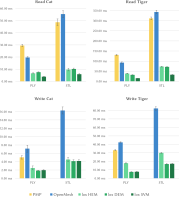
\includegraphics[width=1.1\textwidth]{svg2pdf/io-bench}
  }
  \vspace{1cm}
  \caption{
    Results of the IO benchmarks.
    The height of the bars is the mean of all measurements, the error bar displays the standard deviation.
    Values for \enquote{Write STL} benchmarks are missing for PMP, because the library only supports ASCII STL which is a lot slower than binary STL (those benchmarks took 500\,ms for \emph{cat} and 2000\,ms for \emph{tiger}).
  }
  \label{fig:io-benchmark}
\end{figure}

\newpage

foo
